\documentclass{article}
%\documentclass[journal]{IEEEtran}
%\documentclass{report}
%\documentclass{acta}

\usepackage{graphicx}

\begin{document}

\title{Efficient Policy Enforcement in Android Applications with Counterexample-Guided Abstraction Refinement}
\author{Yu Feng}

\maketitle

\begin{abstract}
In our previous work, we presented Apposcopy~\cite{apposcopy}, a new semantics-based approach 
for identifying a prevalent class of Android malware that steals 
private user information. However, in practice, we also noticed 
that several malicious behaviors can only be triggered under a 
certain sequential system events and our current tool will generate 
several false positives in those cases. To detect such behaviors, 
one way is to perform model checking on the abstract state 
machine of a given Android application.
But the downside is that the system will take a longer time to analyze
a single application. 

To detect malware that violate the security policy specified by users 
in terms of temporal formulas in a efficient way, we apply 
counterexample-guided abstraction refinement-based(CEGAR) model 
checking. The intuition is, we build the TICCG(Temporal Inter-Component 
communication Call Graph) which is the abstract state machine of a given 
Android applicaton, then the system will check the validity of the application
with respect to a set of temporal properties. If it's valid, then 
our system satisfies current properties. If it's invalid, it could
be (1) a true violation, which we report it to the user; Or (2)
a false positive. In this case, we will refine the TICCG based on
the counterexample generated by the trace of system events.
\end{abstract}


\section{Introduction}
As the most popular mobile operating system, the Android platform 
is a growing target for  mobile malware.
Today, many of the malicious applications that afflict  Android users  exploit
the private and monetized information
stored in a user's smartphone, such as the user's contacts, photos, or
account information. 

To mitigate the above problems, researchers have been working on either 
static analysis-based techniques, such as semantic-based approaches and taint analysis, 
or dynamic analysis based on monitoring the execution traces of a 
given application. However, there are still corpus of malware that is hard to detect 
by existing technique. According to a recent literature~\cite{pegasus}, there are
several sophisticated Android malware and their malcious behaviors can only 
be triggered under a specific event sequences. Such malicious behaviors 
are difficult to categorize by simply checking whether they are stealing 
some sensitive informantion. Applications related to audio and video eavedropping 
belong to this spectrum: The malware will record audio and video information
without user's notice through a backgroud process. Traditional way to 
mitigate this problem is to mark both audio and video record as sensitive
data and perform a sound taint analysis on it. 
Unfortunately, since many benign apps  also need access to audio and video record 
to perform their advertised functionality, not every app that
leaks user information can be classified as malware. We need to figure out
a way to differentiate the benign and malicious behaviors to reduce false positives.

In response to the  rapid dissemination of 
Android malware, one alternative approach is to build an abstract
model for Android applications and perform model checking with respect
to the custom specification in the form of temporal formulas. 
Latest work like Pegasus\cite{pegasus} models Android applications as "Permission Event Graph"
and checking the safty properties encoded by Java program. While it can 
differentiate benign applicaton and malicious application through a set 
of safty properties, it also suffers the performance issue: Most of the 
applications will take more than 1000 seconds to terminate. 

The intuition behind our work is that not only do we need to detect
the difference between user expectation and malicious intent through the 
context where system's API and permissions are used during runtime like 
Pegasus~\cite{pegasus},  we should also apply the technique of  
counterexample-guided abstraction refinement-based(CEGAR) to reduce 
the overhead of model checking.

\subsection{Problem and Approach}
Here we describe the challenges behind our approaches in a bit more detail
as well as the insights behind our solutions.

{\bf \emph{Problem Definition}}. Here, we consider the following problems
which are closely related to each other. The first problem is how to design
a specification language to encode the semantic of the event-driven behaviors 
of Android System. Pegasus~\cite{pegasus} expresses the specification 
in terms of Java program and it is not very convenient and compact from the
perspective of the users; The second problem is how to contruct an abstract
model for the interaction between an Android application and the Android
core event system; The last problem is given an abstract model and a specification
in the form of temporal properties, how do we perform model checking efficiently.

{\bf \emph{Challenges}}. Our specification language should be able to 
express some custom security policies that monitor the usage of system API and 
permission in a concise and compact way. For instance, specifying a SMS messge
can not be sent if user does not press the 'SEND' button. Likewise, 
a Device ID can not be uploaded to a remote server if a confirmation 
dialog does not show and confirm by the user.

Even though model checking is a powerful technique for checking the temporal 
properties of Android application, the interaction between the Android application
and Android system is very complicated compared to normal Java program: 
It introduces several event-handler as well as  register-callback mechanisms
which are invisible to traditional control flow graph; To make thing harder, 
recent research show that static analysis of event-driven programs turn out 
to be EXPSPACE-hard~\cite{jhala2007}. So our first challenge is how to model the
interaction between Android application and Android core event system.

The second challenge is how do we design an abstraction that can reflect the 
event-driven behavior in Android application concisely. We do not want to 
model the entire Android system because it will be intractable. Moreover,
the usage of standard Java API and Android SDK makes the event system more complicated.

Now that we have both an abstract model for the Android application and 
a specification of the temporal properties, the third challenge is how to 
perform model checking efficiently. 

{\bf \emph{Insights}}. Our first insight is that even though the Android
event system is complicated, the total number of events and the number of 
API that will change the state of the abstract model is finite. Thus it is
feasible to design a specification language to express the temporal properties
with respect to some security policies. 

Our second insight is that to come up with an abstract model which reflects
the interaction between the Android application and the Android core event 
system, we use a graph to express it explicitly. More specifically, we 
design TICCG(Temporal Inter-Component Communication Call Graph), which is
an extension of our previous ICCG(Inter-Component Communication Call Graph)~\cite{apposcopy}.
More importantly, TICCG abstracts the interactions among the Android event
system, permissions and API usage in the application but ignore the low
level details which is irrelevant to our analysis.

Our third insight is to use the technique of the counterexample-guided 
abstraction refinement-based(CEGAR) to improve the performance of 
model checking. Recent research like JAM\cite{cegar12} introduces CEGAR 
to reduce the runtime overhead of web application in the context of 
Javascript, which is closed to our current work.
To the best of our knowledge, there is no previous model checking tools for 
Android applications which can scale in large applications.

\subsection{Content and Contributions}
The main contributions of this work can be summarized as follows.
% itemize
\begin{itemize}
\item {\bf \emph{TICCG}}, a new abstraction for Android application
that models the temporal behaviors of system APIs and system events;
\item {\bf \emph{Encoding benign and malicious intent}}, we provide a specification
language for user to express the temporal properties of TICCG; 
\item {\bf \emph{TICCG Construction and Analysis}}, we construct TICCG by combining 
traditionl static analyses technique(Pointer analysis, Call Graph construction, taint analysis, etc)
with the semantic of Android API, permission and event system. Then we implement
model checking on TICCG with respect to the specification;
\item {\bf \emph{CEGAR-based refinement}}, We apply the counterexample-guided 
abstraction refinement-based(CEGAR) technique in Android application 
and use it to improve the performance of the system dramatically.
\item {\bf \emph{Experiments}}, We run our tool on both some benign applications and 
malware to verify that our system can identify malicious behaviors precisely.
\end{itemize}

The paper is structured as follows: We first provide some background knowledge of
Android framework and illustrate our technique by a simple example in Section~\ref{sec:overview}.
Secondly we formalize the definition of TICCG in Section~\ref{sec:ticcg} and 
the algorithm to construct it in Section~\ref{sec:construct}. Third, 
we describe some details about our refinement with CEGAR in Section~\ref{sec:cegar}, 
followed by our preliminary evaluation in Section~\ref{sec:eval}.
Finally we conclude our work in Section~\ref{sec:conclude}.

\section{Background and Overview}
\label{sec:overview}
In this section, we will first introduce some basic knowledge of Android framework 
and then illustrate our approach using a simplified version of a malcious application.

\subsection{Android Background}
\begin{itemize}
\item {\bf \emph{Components}}. An Android application consists of four kinds of components, 
\emph{Activity}, \emph{Service}, \emph{BroadcastReceiver}, and \emph{ContentProvider}.
Activity components form the basis of the user
  interface, and each window of the application is typically controlled by
  an activity. Service components run in the background and remain active even
  if windows are switched. 
  %Services can expose interfaces for communication with other applications.
BroadcastReceiver components react asynchronously to messages
  from other applications. Finally, ContentProvider components store data relevant to the
  application, usually in a database, and allow sharing  data across applications.

\item {\bf \emph{Permissions}}. A security \emph{permission} that can be used to 
put the limitation on the access of some system resources. Typically, an application
needs specific permissions to access SMS message, contact list, SD card, etc.

\item {\bf \emph{Lifecycle methods}}. A special set of pre-defined methods which is used 
to manage the lifecycle of Android components. As a user navigates though, pause and switch
out of current application, different lifecycle methods will be invoked to switch the 
component to different states. For instance, an application might call \emph{startActivity}
to start an Activity. When the user switch out to other application and then switch back again,
\emph{onResume} method will be invoked by the Android system automatically.  

\item {\bf \emph{System APIs and Events}}. Those are two way for an application to communicate
with the Android system. A typical scenario in Android application is: the programmer will define
callbacks and add hook them up to some events through listeners. As soon as the event is fired, 
its corresponding callback method will be invoked by the Android system. For instance, 
SMS Received notification, Phone calls, etc.

\end{itemize}

\subsection{System Overview}
% Figure
\begin{figure}
\centerline{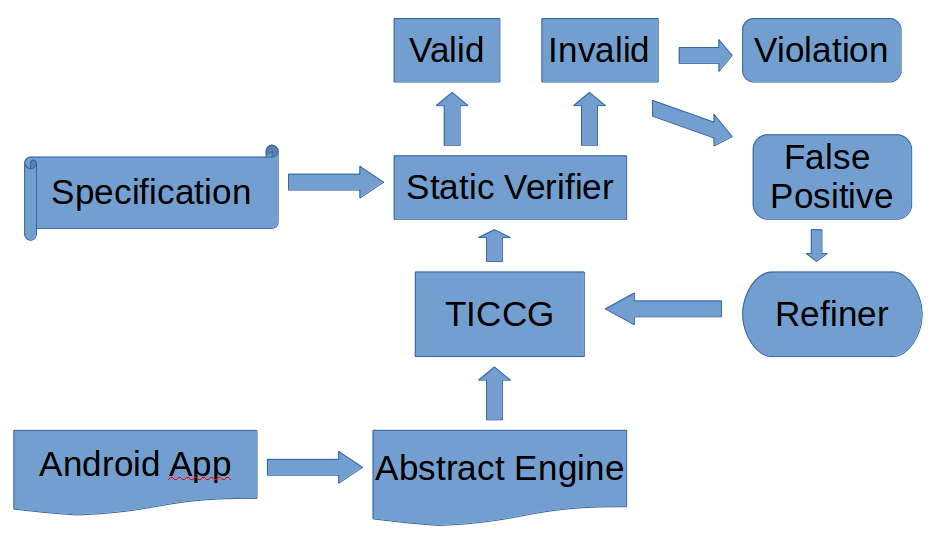
\includegraphics[scale=0.4]{sysgraph}}
\caption{System Overview}
\label{fig:one}
\end{figure}

Figure~\ref{fig:one} shows an overview of the system architecture.
It takes as input an Android application(source code or bytecode) 
and a set of temporal properties encoded as datalog. By running the 
abstract engine, the system first converts the Android application 
to TICCG(Temporal Inter-Component Communication Call Graph), 
which is the augmented version of our previous work\cite{apposcopy}
by modeling the system events and system APIs in the graph. 
Then the static verifier will perform stardard model checking to 
verify whether all the temporal properties are valid with respect 
to a given TICCG. If the result is valid and since our analysis is 
sound, we conclude that current application will not violate those
temporal properties. If the result is invalid, then there exists two
cases: (1) We detect a true violation and report it to the user; 
(2) It is a false positive because our analysis is imprecise or the 
given temporal formulas are too strong to exclude some benign applications.
For the first case, we will use current system event traces as a counterexample
\cite{clarkecegar} and  run the refiner to refine the original 
TICCG to prune the search space; For the second case, we can manully
modify the temporal formulas based on some domain specific information.

\subsection{Our approach by Example}
In the section we will briefly illustrate our approach using a simplified 
version of a malcious application.

Figure~\ref{dropcall} is a malware named "Drop Call". It it a typical 
eavesdropping malware which records audios silently without interacting with the
User Interface of the application. If we mark audio record as sensitive data 
and perform traditional taint analysis in a naive way, we might also 
exclude a lot of legitimate applications. A typical benigh usage of this 
application should be: 

\begin{figure}[ht!]
\centering
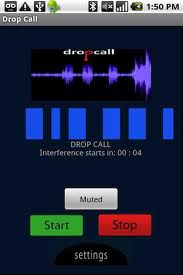
\includegraphics[scale=0.8]{dropped-call.jpg}
\caption{Drop Call example\label{dropcall}}
\end{figure}


\section{Our Abstraction for Android Application}
\label{sec:ticcg}

\section{TICCG Construction}
\label{sec:construct}

\section{Abstract Refinement}
\label{sec:cegar}

\section{Evaluation}
\label{sec:eval}

\section{Conclusion}
\label{sec:conclude}

% Bibliography
%\bibliographystyle{ACM-Reference-Format-Journals}
%\bibliography{mybib}
\bibliography{ctl}
\bibliographystyle{plain}
 

\end{document}
